The people that use a system can be represented by personas. This is done in order to ensure the PACT elements are centred in the design process. Personas are general profiles of different types of users. A persona is a concrete representation of a fictitious person. Personas help the designer by having a specific end user in mind, preventing them designing the system for themselves. Personas are developed through the understanding process and through undertaking a PACT analysis. A part of the persona is a short story of the person trying to achieve a goal using the system in a specific context~\cite{benyon2013designing}.

As part of this project, three personas were made. The personas was made by following the 10 step process described in~\cite{nielsen2007persona}. Here follows a description of each of the steps and how they were conducted in this project.

\subsubsection{Step 1: Finding the Users}
In this step general information about the users as a group is gathered. It should be determined how many users there are and in which ways they will be using the product. This is done by gathering primarily quantitative data from interviews, observations, second hand information, questionnaires and reports~\cite{nielsen2007ten}. When the persona creation process started, some prior knowledge about users was already present based on experiences by the authors of this report. To extend this knowledge interviews were conducted as described in~\cref{userInterviews}.

\subsubsection{Step 2: Building a Hypothesis}
In this step it is analysed how the users are different and based on this split into different groups. This is done using the material gathered in step 1. In this report, the users were divided into two groups: staff at venues and guests at venues.

\subsubsection{Step 3: Verification}
In verification the focus is on finding data that supports the initial hypothesis found in step 2. This will later support the personas descriptions and the scenario writing. This is also the step where you go more in depth with the users. What do they dislike, what are their values, what are their attitudes towards the system/site and in what conditions will they use the system/site? This data is then compared to the data from step 2. To find any potential flaws or new groups of users.

After doing this step it was found that there were two kinds of users, the ones that already requested music at venues and the ones that did not.

\subsubsection{Step 4: Finding Patterns}
This is where you categorise the users based on the initial separation from step 2. Are the groups right?

After this step three distinct groups were formed:
\begin{enumerate}
    \item Active users requesting songs
    \item Passive users
    \item Bartenders
\end{enumerate}

\subsubsection{Step 5: Constructing Personas}
This is the step where the actual personas are created. Based on the patterns found in step 4 one persona representing each group is made. This is done with narrative techniques to tell a story about a person. It is important not to come up with stereotypes, but with realistic persons that people can relate to. Some information can be based on actual data while other information can be made up to fill in the gaps. According to~\cite{nielsen2007persona} it is important that as many people are involved in the process of creating personas. The personas for the project was done as a collaboration between the whole group. The three resulting personas can be seen in \cref{akkpersona}.

\subsubsection{Step 6: Defining Situations}
In this step the needs of the personas are identified and situations in which the persona will use the product is described.

Based on prior data collected in interviews, observations and experiences, a list of situations in which the product will we used and the associated needs is created.

\subsubsection{Step 7: Validation and Buy-in}
In this step the personas are validated by someone not involved in the creation process. This will result in a list of corrections. In this project a person not involved got to read the personas and give comments, this led to minor adjustments.

\subsubsection{Step 8: Dissemination of Knowledge}
In this step you have to consider how to get the information from the personas out to the developers and designers that needs to use them. Since this project is done by a small group this was not a big problem. The personas were printed out and places in our work space, easy accessible for everyone.

\subsubsection{Step 9: Creating Scenarios}
In this step it is described what happens when a user uses the product with a goal in mind. This will be based on the persona from step 5 and situations from step 6. The resulting persona with scenario can be seen in \cref{akkpersona}. This step will also result in use cases, found in \cref{usecase}.

\subsubsection{Step 10: Ongoing Development}
The last step is an ongoing step where you update the information if needed. This can happen when there is new data showing something not considered before. After the interviews with with the bar described in \cref{sec:fabrikken}, the personas was updated to have a clearly defined persona representing a bartender.

\section{Personas in The Project}
\label{akkpersona}

Based on the steps defined in \cref{persona}, three personas are
defined to help in keeping the users of the system in mind.

\subsection{Camilla}
\begin{figure}[hbtp]
  \centering
  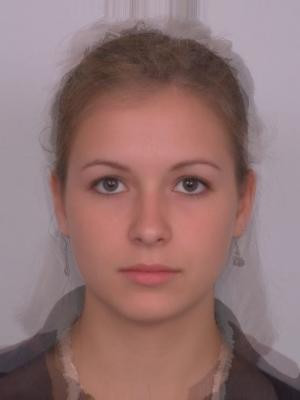
\includegraphics[]{camilla.jpg}
  \caption{Picture associated with the persona \enquote{Camilla}. Copyright the Face Research Lab. Used with permission.}\label{fig:camilla}
\end{figure}
\noindent\textbf{Basic information}

\begin{itemize}
\item 20 years old
\item Medical student
\item Employed in an elderly care centre
\item She loves meeting new people
\item When going out she likes to visit small places that allow socialisation
\item Volunteered in Red Cross Uganda
\item Frequent user of her smartphone, but does not consider herself as an expert at technology
\end{itemize}

It is Friday afternoon and Camilla is planning to meet some of her fellow students at a bar. Camilla and her friends get together after they are finished at school and go to a café to grab a sandwich. After dinner, Camilla takes out her smartphone and checks openPlaylist. Camilla can see that some of her favourite tracks are being played at White Hart, and they agree to go there. Upon arriving Camilla checks in via the application. She immediately notices on the screen behind the bar that the queue is filled with tracks she dislikes. She now uses the application to request and upvote other tracks that she would like to be played. Some other people at White Hart agree on Camilla's choices and they too upvote these tracks. On the screen in the bar Camilla can see some of the other people that upvotes her tracks and later in the evening she meets them and they talk about all the nice music they have in common. Camilla and her new and old friends party all night long and drink a lot of beer. \jenote{Godt nok sprog? Det kan måske lige gøres lidt mere professionelt}

\subsection{Mathias}
\begin{figure}[hbtp]
  \centering
  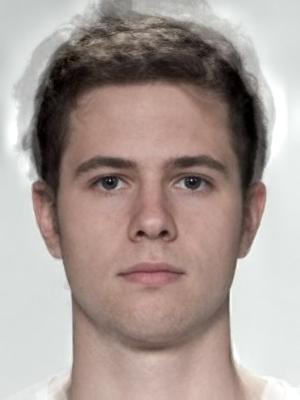
\includegraphics[]{mathias.jpg}
  \caption[Persona \enquote{Mathias}.]{Picture associated with the persona \enquote{Mathias}. Copyright the Face Research Lab. Used with permission.}\label{fig:mathias}
\end{figure}

\subsubsection{Basic information}
\begin{itemize}
\item 21 years old
\item Mechanical engineering student
\item Introvert
\item Thoughtful person that can be shy at times
\end{itemize}

\subsubsection{Scenario}
Mathias is intelligent, logical and not very good with social interaction. Mathias, like most of his peers, likes going to a bar and having a beer or two after a productive week and this week was going to be no different. Mathias goes to his favourite bar, but soon finds that the music is not fitting to his mood. Normally, this would be a deal breaker for Mathias, and he would find another bar for the night, as he was not really comfortable going to the bartender and requesting music he likes. Fortunately Mathias had just learned about openPlaylist. Mathias opens the mobile application and finds that it is only the next couple of tracks that he dislikes, so he decides to vote for tracks which he does like and stays at the bar after all.

\subsubsection{Adam}
\begin{figure} [h]
  \centering
  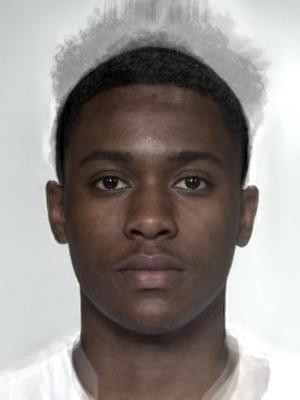
\includegraphics[]{adam.jpg}
  \caption{Picture associated with the persona \enquote{Adam}. Copyright the Face Research Lab. Used with permission.}\label{fig:adam}
\end{figure}
\noindent\textbf{Basic information}

\begin{itemize}
\item 23 years old
\item Works as a bartender in central Aalborg
\item Likes socialising and talking to people
\item Not afraid to try new technology
\end{itemize}

Adam has just begun his night shift in the bar. Usually Adam would have to manage the bars music system, as well as tend the bar, until the DJ arrives, but not tonight. The bar has just yesterday implemented openPlaylist. Now, when people come up to Adam to request tracks, he can just tell them about the openPlaylist app. With Adam not having to manage the music system manually, the queue to the bar has never been shorter.

